Mentre nella fotometria si ha soltanto una distribuzione di flusso (che potrebbe essere anche falsata, abbiamo visto ad esempio che il mezzo interstellare tende ad arrossare gli oggetti), nella spettroscopia si usano le righe spettrali, che sono quelle che ci servono per capire quando due stelle sono uguali. L'obbiettivo della spettroscopia è quello di distinguere le lunghezze d'onda, ma non come abbiamo visto fin'ora in delle bande grandi 1500 \AA, bensì su scale molto più piccole dove andiamo a vedere piccole bande di assorbimento e da queste capiamo ad esempio com'è fatta l'atmosfera di una stella.

\subsection{Spettrografi}

Per poter far questo ci serve una capacità di distinguere i colori altissima, cioè bisogna essere in grado di separare le lunghezze d'onda con un'elevata precisione. Per fare questo usiamo gli spettrografi, i quali sfruttano il fenomeno della dispersione che subisce la luce quando attraversa un prisma (detto anche dispersore).

Immaginiamo di dover registrare ogni singolo colore in un pixel, come se fosse una fotografia, solo che adesso nella foto avremo la stessa stella nei suoi colori. Quello che ci serve è un sistema per disperdere (separare spazialmente) i colori, in modo tale che su ogni pixel abbiamo solo un piccolo intervallo di lunghezze d'onda. Questa cosa non è così semplice da realizzare, perché quando andiamo a fare una foto di una stella col telescopio, pur supponendo che questa emetta una sola frequenza (cioè sia monocromatica), quello che otteniamo non è un oggetto puntiforme, quindi che occupa un singolo pixel, ma, per come abbiamo costruito il telescopio, questa avrà nel piano focale una certa dimensione in pixel\footnote{Ricordiamo che il telescopio si comporta come una fenditura, per cui quando arriva il fronte d'onda produce una figura di interferenza.}. Quello che si fa allora è combinare due parametri di uno spettrografo:

\begin{itemize}
   \item La separazione spaziale, cioè lo strumento deve disperdere i colori. Infatti quando la luce attraversa il prisma, i raggi aventi diversi colori escono con angoli diversi dal prisma, però ognuno di queste lunghezze d'onda produce sul piano focale delle immagini di interferenza;

   \item La larghezza dei picchi, questi infatti devono restare stretti.
\end{itemize}

Questi due parametri sono quelli fondamentali. In analogia a quanto fatto col potere risolutivo, possiamo adottare il criterio di Rayleigh (il quale afferma che due stelle sono distinte se la loro immagine è tale che lo zero di una cada in corrispondenza del massimo dell'altra, ovvero se le full width half maximum cioè la larghezza a metà altezza sono completamente distinte) per i colori. In questo caso possiamo definire un parametro, detto \textit{potere risolutivo} degli spettroscopi, dato dal rapporto tra la lunghezza d'onda considerata diviso la larghezza di quella lunghezza d'onda nel piano focale, cioè:

$$R=\frac{\lambda}{\Delta \lambda}$$

Questo valore è solitamente, per gli astronomi, di $10^5 - 10^6$. Questo risultato si può ottenere attraverso l'interferenza, cioè mettendo un gran numero di fenditure molto piccole, vicine tra loro. Da questa otteniamo l'immagine di interferenza da cui estraiamo le informazioni che ci servono.

Una migliore risoluzione ottica può permetterci ad esempio di calcolare la velocità di stelle o pianeti sfruttando l'effetto doppler. Sappiamo infatti che quando la sorgente che emette luce si muove con una certa velocità $v$, la lunghezza d'onda della luce emessa cambia secondo la legge:

$$\frac{\Delta \lambda}{\lambda} = \frac{v}{c}$$

dove $\lambda$ è la lunghezza d'onda che la sorgente avrebbe se fosse ferma e $\Delta \lambda$ invece è la variazione della lunghezza d'onda stessa. Nel caso in cui il nostro spettrografo sia in grado di distinguere la variazione di lunghezza d'onda possiamo calcolare la velocità con cui si muove la sorgente (ovviamente soltanto la velocità parallela alla direzione di osservazione, non quella ortogonale). Non è sempre detto che questa sia possibile, infatti in base al potere risolutivo del nostro strumento può capitare che il picco si sposti all'interno di uno stesso pixel e quindi non ci accorgiamo dello spostamento del picco.

Cerchiamo di capire un po' meglio quanti fotoni necessitano questi strumenti. Sappiamo, dall'esperimento delle fenditure (tipo reticolo), che al centro delle fenditure i picchi sono più larghi mentre man mano che ci si allontana dal centro (si dice che si va a ordini maggiori) i picchi sono sempre più piccoli e quindi è più facile distinguere le diverse lunghezze d'onda. Allo stesso tempo però il picco è anche meno evidente perché il numero di fotoni che arriva in quelle zone è piccolo. 

Il problema del sistema tipo quelli che abbiamo visto riguarda l'efficienza, cioè non tutti gli elettroni che arrivano nel prisma passano. Inoltre dobbiamo considerare anche l'interferenza di quelli che passano. Consideriamo ad esempio l'esperimento delle fenditure: se facciamo passare una luce policromatica, si avrà che al centro tutti i fotoni interferiscono costruttivamente, quindi si ha una sovrapposizione di picchi, che non è utile ai nostri scopi. Per avere una buona separazione bisogna andare ad ordini maggiori rispetto al primo, detto di ordine zero (bisogna in pratica spostarsi di lato, si pensi al prisma/reticolo studiato a lab 2), ad esempio per avere una risoluzione di 100000 dovremmo andare almeno all'ordine 100. Lo svantaggio però è che salendo l'ordine diminuisce l'efficienza, poiché un numero molto piccolo di fotoni arriva nelle zone laterali del nostro schermo (ricordiamo che lo schermo deve essere piatto), all'ordine cento sarebbe pressoché zero. L'alta efficienza degli strumenti moderni è stata raggiunta utilizzando un pezzo di vetro plasmato a forma di gradini e rivestito di alluminio. In questo modo l'interferenza è tra le facce che riflettono nella stessa direzione, come per le fenditure (nel senso che l'interferenza si ha per le fenditure nella medesima direzione) e questo fa si che il picco maggiore di luce non è più al centro, come ad esempio per le fenditure, ma si trovi proprio negli ordini alti, portando l'efficienza da un valore molto basso ad un valore che è quasi pari a quello massimo.

\begin{figure}[H]
  \centering
  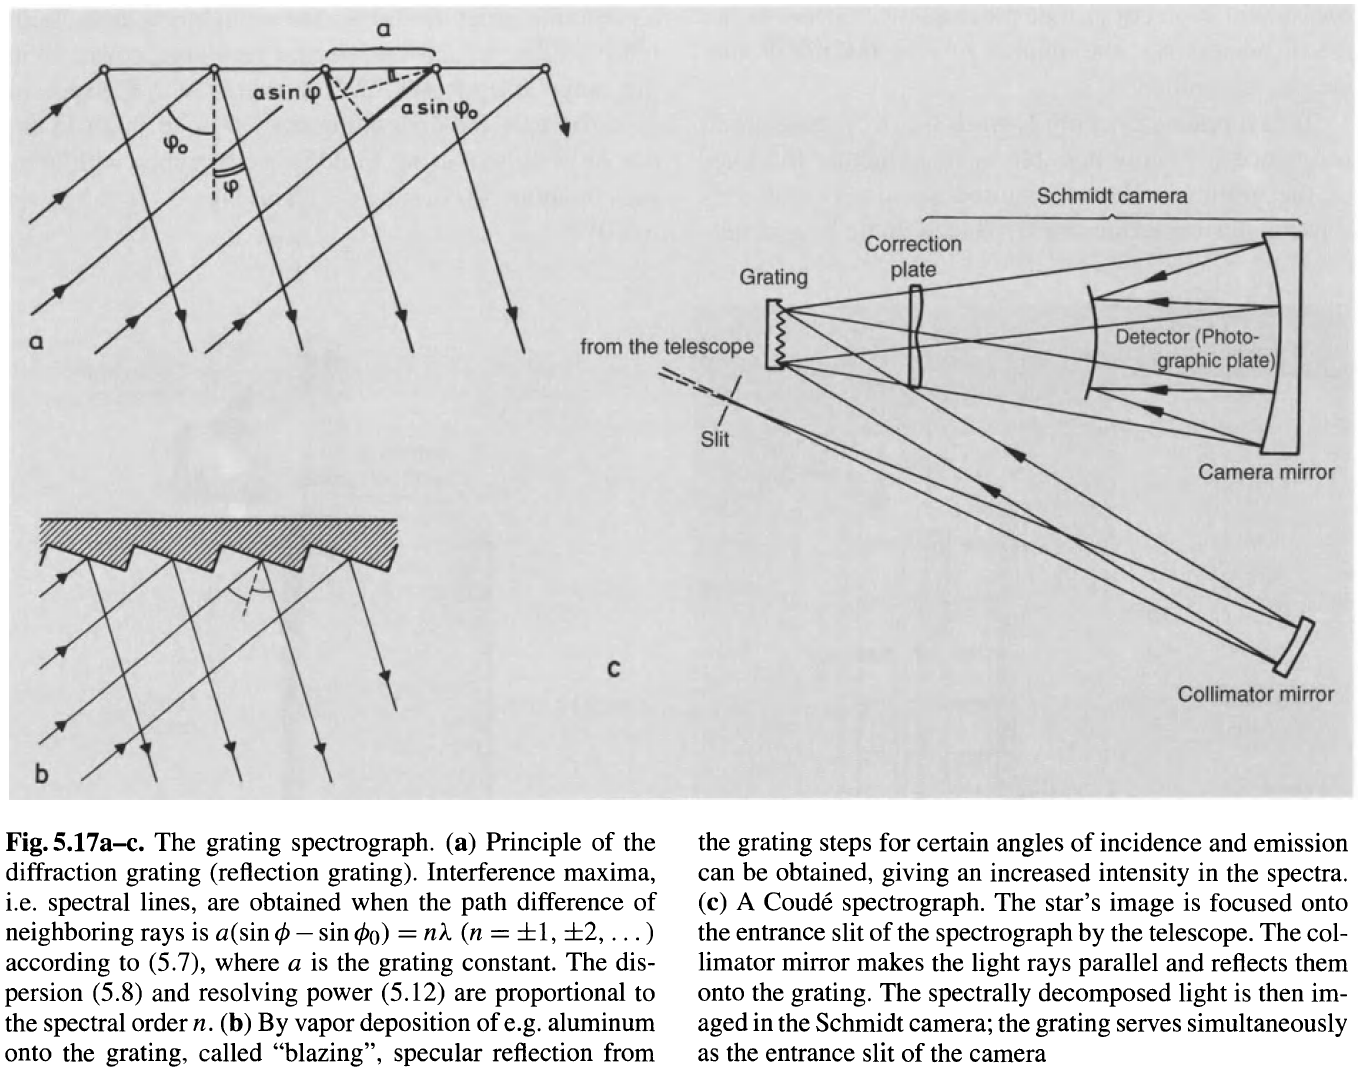
\includegraphics[width=\textwidth]{immagini/spettrografo_a_gradino.png}
\end{figure}


